% Created by tikzDevice version 0.12.6 on 2026-02-05 15:03:40
% !TEX encoding = UTF-8 Unicode
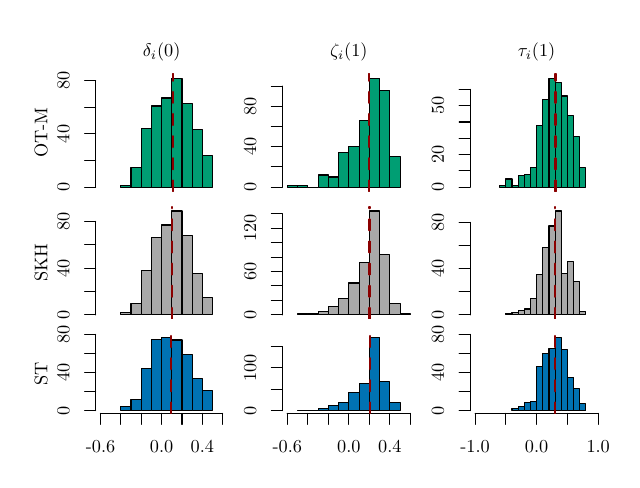
\begin{tikzpicture}[x=1pt,y=1pt]
\definecolor{fillColor}{RGB}{255,255,255}
\path[use as bounding box,fill=fillColor,fill opacity=0.00] (0,0) rectangle (211.10,156.03);
\begin{scope}
\path[clip] ( 24.55, 96.84) rectangle ( 72.23,139.40);
\definecolor{drawColor}{RGB}{0,0,0}
\definecolor{fillColor}{RGB}{0,158,115}

\path[draw=drawColor,line width= 0.4pt,line join=round,line cap=round,fill=fillColor] ( 33.67, 98.41) rectangle ( 37.35, 98.89);

\path[draw=drawColor,line width= 0.4pt,line join=round,line cap=round,fill=fillColor] ( 37.35, 98.41) rectangle ( 41.03,105.62);

\path[draw=drawColor,line width= 0.4pt,line join=round,line cap=round,fill=fillColor] ( 41.03, 98.41) rectangle ( 44.71,119.56);

\path[draw=drawColor,line width= 0.4pt,line join=round,line cap=round,fill=fillColor] ( 44.71, 98.41) rectangle ( 48.39,127.73);

\path[draw=drawColor,line width= 0.4pt,line join=round,line cap=round,fill=fillColor] ( 48.39, 98.41) rectangle ( 52.07,130.61);

\path[draw=drawColor,line width= 0.4pt,line join=round,line cap=round,fill=fillColor] ( 52.07, 98.41) rectangle ( 55.75,137.82);

\path[draw=drawColor,line width= 0.4pt,line join=round,line cap=round,fill=fillColor] ( 55.75, 98.41) rectangle ( 59.42,128.69);

\path[draw=drawColor,line width= 0.4pt,line join=round,line cap=round,fill=fillColor] ( 59.42, 98.41) rectangle ( 63.10,119.08);

\path[draw=drawColor,line width= 0.4pt,line join=round,line cap=round,fill=fillColor] ( 63.10, 98.41) rectangle ( 66.78,109.95);
\end{scope}
\begin{scope}
\path[clip] (  0.00,  0.00) rectangle (211.10,156.03);
\definecolor{drawColor}{RGB}{0,0,0}

\path[draw=drawColor,line width= 0.4pt,line join=round,line cap=round] ( 24.55, 98.41) -- ( 24.55,136.86);

\path[draw=drawColor,line width= 0.4pt,line join=round,line cap=round] ( 24.55, 98.41) -- ( 20.59, 98.41);

\path[draw=drawColor,line width= 0.4pt,line join=round,line cap=round] ( 24.55,108.02) -- ( 20.59,108.02);

\path[draw=drawColor,line width= 0.4pt,line join=round,line cap=round] ( 24.55,117.64) -- ( 20.59,117.64);

\path[draw=drawColor,line width= 0.4pt,line join=round,line cap=round] ( 24.55,127.25) -- ( 20.59,127.25);

\path[draw=drawColor,line width= 0.4pt,line join=round,line cap=round] ( 24.55,136.86) -- ( 20.59,136.86);

\node[text=drawColor,rotate= 90.00,anchor=base,inner sep=0pt, outer sep=0pt, scale=  0.66] at ( 15.05, 98.41) {0};

\node[text=drawColor,rotate= 90.00,anchor=base,inner sep=0pt, outer sep=0pt, scale=  0.66] at ( 15.05,117.64) {40};

\node[text=drawColor,rotate= 90.00,anchor=base,inner sep=0pt, outer sep=0pt, scale=  0.66] at ( 15.05,136.86) {80};
\end{scope}
\begin{scope}
\path[clip] (  0.00, 92.08) rectangle ( 75.39,156.03);
\definecolor{drawColor}{RGB}{0,0,0}

\node[text=drawColor,anchor=base,inner sep=0pt, outer sep=0pt, scale=  0.66] at ( 48.39,145.44) {\bfseries $\delta_i(0)$};

\node[text=drawColor,rotate= 90.00,anchor=base,inner sep=0pt, outer sep=0pt, scale=  0.66] at (  7.13,118.12) {OT-M};
\end{scope}
\begin{scope}
\path[clip] ( 24.55, 96.84) rectangle ( 72.23,139.40);
\definecolor{drawColor}{RGB}{139,0,0}

\path[draw=drawColor,line width= 0.8pt,dash pattern=on 4pt off 4pt ,line join=round,line cap=round] ( 52.50, 96.84) -- ( 52.50,139.40);
\end{scope}
\begin{scope}
\path[clip] ( 92.03, 96.84) rectangle (140.08,139.40);
\definecolor{drawColor}{RGB}{0,0,0}
\definecolor{fillColor}{RGB}{0,158,115}

\path[draw=drawColor,line width= 0.4pt,line join=round,line cap=round,fill=fillColor] ( 93.80, 98.41) rectangle ( 97.51, 99.14);

\path[draw=drawColor,line width= 0.4pt,line join=round,line cap=round,fill=fillColor] ( 97.51, 98.41) rectangle (101.22, 99.14);

\path[draw=drawColor,line width= 0.4pt,line join=round,line cap=round,fill=fillColor] (101.22, 98.41) rectangle (104.93, 98.41);

\path[draw=drawColor,line width= 0.4pt,line join=round,line cap=round,fill=fillColor] (104.93, 98.41) rectangle (108.64,102.79);

\path[draw=drawColor,line width= 0.4pt,line join=round,line cap=round,fill=fillColor] (108.64, 98.41) rectangle (112.34,102.06);

\path[draw=drawColor,line width= 0.4pt,line join=round,line cap=round,fill=fillColor] (112.34, 98.41) rectangle (116.05,110.82);

\path[draw=drawColor,line width= 0.4pt,line join=round,line cap=round,fill=fillColor] (116.05, 98.41) rectangle (119.76,113.01);

\path[draw=drawColor,line width= 0.4pt,line join=round,line cap=round,fill=fillColor] (119.76, 98.41) rectangle (123.47,122.50);

\path[draw=drawColor,line width= 0.4pt,line join=round,line cap=round,fill=fillColor] (123.47, 98.41) rectangle (127.18,137.82);

\path[draw=drawColor,line width= 0.4pt,line join=round,line cap=round,fill=fillColor] (127.18, 98.41) rectangle (130.88,133.44);

\path[draw=drawColor,line width= 0.4pt,line join=round,line cap=round,fill=fillColor] (130.88, 98.41) rectangle (134.59,109.36);
\end{scope}
\begin{scope}
\path[clip] (  0.00,  0.00) rectangle (211.10,156.03);
\definecolor{drawColor}{RGB}{0,0,0}

\path[draw=drawColor,line width= 0.4pt,line join=round,line cap=round] ( 92.03, 98.41) -- ( 92.03,134.90);

\path[draw=drawColor,line width= 0.4pt,line join=round,line cap=round] ( 92.03, 98.41) -- ( 88.07, 98.41);

\path[draw=drawColor,line width= 0.4pt,line join=round,line cap=round] ( 92.03,105.71) -- ( 88.07,105.71);

\path[draw=drawColor,line width= 0.4pt,line join=round,line cap=round] ( 92.03,113.01) -- ( 88.07,113.01);

\path[draw=drawColor,line width= 0.4pt,line join=round,line cap=round] ( 92.03,120.31) -- ( 88.07,120.31);

\path[draw=drawColor,line width= 0.4pt,line join=round,line cap=round] ( 92.03,127.61) -- ( 88.07,127.61);

\path[draw=drawColor,line width= 0.4pt,line join=round,line cap=round] ( 92.03,134.90) -- ( 88.07,134.90);

\node[text=drawColor,rotate= 90.00,anchor=base,inner sep=0pt, outer sep=0pt, scale=  0.66] at ( 82.52, 98.41) {0};

\node[text=drawColor,rotate= 90.00,anchor=base,inner sep=0pt, outer sep=0pt, scale=  0.66] at ( 82.52,113.01) {40};

\node[text=drawColor,rotate= 90.00,anchor=base,inner sep=0pt, outer sep=0pt, scale=  0.66] at ( 82.52,127.61) {80};
\end{scope}
\begin{scope}
\path[clip] ( 75.39, 92.08) rectangle (143.25,156.03);
\definecolor{drawColor}{RGB}{0,0,0}

\node[text=drawColor,anchor=base,inner sep=0pt, outer sep=0pt, scale=  0.66] at (116.05,145.44) {\bfseries $\zeta_i(1)$};
\end{scope}
\begin{scope}
\path[clip] ( 92.03, 96.84) rectangle (140.08,139.40);
\definecolor{drawColor}{RGB}{139,0,0}

\path[draw=drawColor,line width= 0.8pt,dash pattern=on 4pt off 4pt ,line join=round,line cap=round] (123.26, 96.84) -- (123.26,139.40);
\end{scope}
\begin{scope}
\path[clip] (159.88, 96.84) rectangle (207.93,139.40);
\definecolor{drawColor}{RGB}{0,0,0}
\definecolor{fillColor}{RGB}{0,158,115}

\path[draw=drawColor,line width= 0.4pt,line join=round,line cap=round,fill=fillColor] (170.56, 98.41) rectangle (172.78, 99.00);

\path[draw=drawColor,line width= 0.4pt,line join=round,line cap=round,fill=fillColor] (172.78, 98.41) rectangle (175.01,101.35);

\path[draw=drawColor,line width= 0.4pt,line join=round,line cap=round,fill=fillColor] (175.01, 98.41) rectangle (177.23, 99.00);

\path[draw=drawColor,line width= 0.4pt,line join=round,line cap=round,fill=fillColor] (177.23, 98.41) rectangle (179.46,102.53);

\path[draw=drawColor,line width= 0.4pt,line join=round,line cap=round,fill=fillColor] (179.46, 98.41) rectangle (181.68,103.12);

\path[draw=drawColor,line width= 0.4pt,line join=round,line cap=round,fill=fillColor] (181.68, 98.41) rectangle (183.91,105.47);

\path[draw=drawColor,line width= 0.4pt,line join=round,line cap=round,fill=fillColor] (183.91, 98.41) rectangle (186.13,120.76);

\path[draw=drawColor,line width= 0.4pt,line join=round,line cap=round,fill=fillColor] (186.13, 98.41) rectangle (188.36,130.18);

\path[draw=drawColor,line width= 0.4pt,line join=round,line cap=round,fill=fillColor] (188.36, 98.41) rectangle (190.58,137.82);

\path[draw=drawColor,line width= 0.4pt,line join=round,line cap=round,fill=fillColor] (190.58, 98.41) rectangle (192.80,136.06);

\path[draw=drawColor,line width= 0.4pt,line join=round,line cap=round,fill=fillColor] (192.80, 98.41) rectangle (195.03,131.35);

\path[draw=drawColor,line width= 0.4pt,line join=round,line cap=round,fill=fillColor] (195.03, 98.41) rectangle (197.25,124.29);

\path[draw=drawColor,line width= 0.4pt,line join=round,line cap=round,fill=fillColor] (197.25, 98.41) rectangle (199.48,116.65);

\path[draw=drawColor,line width= 0.4pt,line join=round,line cap=round,fill=fillColor] (199.48, 98.41) rectangle (201.70,105.47);
\end{scope}
\begin{scope}
\path[clip] (  0.00,  0.00) rectangle (211.10,156.03);
\definecolor{drawColor}{RGB}{0,0,0}

\path[draw=drawColor,line width= 0.4pt,line join=round,line cap=round] (159.88, 98.41) -- (159.88,133.71);

\path[draw=drawColor,line width= 0.4pt,line join=round,line cap=round] (159.88, 98.41) -- (155.92, 98.41);

\path[draw=drawColor,line width= 0.4pt,line join=round,line cap=round] (159.88,104.29) -- (155.92,104.29);

\path[draw=drawColor,line width= 0.4pt,line join=round,line cap=round] (159.88,110.18) -- (155.92,110.18);

\path[draw=drawColor,line width= 0.4pt,line join=round,line cap=round] (159.88,116.06) -- (155.92,116.06);

\path[draw=drawColor,line width= 0.4pt,line join=round,line cap=round] (159.88,121.94) -- (155.92,121.94);

\path[draw=drawColor,line width= 0.4pt,line join=round,line cap=round] (159.88,127.82) -- (155.92,127.82);

\path[draw=drawColor,line width= 0.4pt,line join=round,line cap=round] (159.88,133.71) -- (155.92,133.71);

\node[text=drawColor,rotate= 90.00,anchor=base,inner sep=0pt, outer sep=0pt, scale=  0.66] at (150.37, 98.41) {0};

\node[text=drawColor,rotate= 90.00,anchor=base,inner sep=0pt, outer sep=0pt, scale=  0.66] at (150.37,110.18) {20};

\node[text=drawColor,rotate= 90.00,anchor=base,inner sep=0pt, outer sep=0pt, scale=  0.66] at (150.37,127.82) {50};
\end{scope}
\begin{scope}
\path[clip] (143.25, 92.08) rectangle (211.10,156.03);
\definecolor{drawColor}{RGB}{0,0,0}

\node[text=drawColor,anchor=base,inner sep=0pt, outer sep=0pt, scale=  0.66] at (183.91,145.44) {\bfseries $\tau_i(1)$};
\end{scope}
\begin{scope}
\path[clip] (159.88, 96.84) rectangle (207.93,139.40);
\definecolor{drawColor}{RGB}{139,0,0}

\path[draw=drawColor,line width= 0.8pt,dash pattern=on 4pt off 4pt ,line join=round,line cap=round] (190.72, 96.84) -- (190.72,139.40);
\end{scope}
\begin{scope}
\path[clip] ( 24.55, 50.79) rectangle ( 72.23, 91.29);
\definecolor{drawColor}{RGB}{0,0,0}
\definecolor{fillColor}{RGB}{169,169,169}

\path[draw=drawColor,line width= 0.4pt,line join=round,line cap=round,fill=fillColor] ( 33.67, 52.29) rectangle ( 37.35, 53.14);

\path[draw=drawColor,line width= 0.4pt,line join=round,line cap=round,fill=fillColor] ( 37.35, 52.29) rectangle ( 41.03, 56.51);

\path[draw=drawColor,line width= 0.4pt,line join=round,line cap=round,fill=fillColor] ( 41.03, 52.29) rectangle ( 44.71, 68.30);

\path[draw=drawColor,line width= 0.4pt,line join=round,line cap=round,fill=fillColor] ( 44.71, 52.29) rectangle ( 48.39, 80.10);

\path[draw=drawColor,line width= 0.4pt,line join=round,line cap=round,fill=fillColor] ( 48.39, 52.29) rectangle ( 52.07, 84.74);

\path[draw=drawColor,line width= 0.4pt,line join=round,line cap=round,fill=fillColor] ( 52.07, 52.29) rectangle ( 55.75, 89.79);

\path[draw=drawColor,line width= 0.4pt,line join=round,line cap=round,fill=fillColor] ( 55.75, 52.29) rectangle ( 59.42, 80.94);

\path[draw=drawColor,line width= 0.4pt,line join=round,line cap=round,fill=fillColor] ( 59.42, 52.29) rectangle ( 63.10, 67.04);

\path[draw=drawColor,line width= 0.4pt,line join=round,line cap=round,fill=fillColor] ( 63.10, 52.29) rectangle ( 66.78, 58.61);
\end{scope}
\begin{scope}
\path[clip] (  0.00,  0.00) rectangle (211.10,156.03);
\definecolor{drawColor}{RGB}{0,0,0}

\path[draw=drawColor,line width= 0.4pt,line join=round,line cap=round] ( 24.55, 52.29) -- ( 24.55, 86.00);

\path[draw=drawColor,line width= 0.4pt,line join=round,line cap=round] ( 24.55, 52.29) -- ( 20.59, 52.29);

\path[draw=drawColor,line width= 0.4pt,line join=round,line cap=round] ( 24.55, 60.72) -- ( 20.59, 60.72);

\path[draw=drawColor,line width= 0.4pt,line join=round,line cap=round] ( 24.55, 69.15) -- ( 20.59, 69.15);

\path[draw=drawColor,line width= 0.4pt,line join=round,line cap=round] ( 24.55, 77.57) -- ( 20.59, 77.57);

\path[draw=drawColor,line width= 0.4pt,line join=round,line cap=round] ( 24.55, 86.00) -- ( 20.59, 86.00);

\node[text=drawColor,rotate= 90.00,anchor=base,inner sep=0pt, outer sep=0pt, scale=  0.66] at ( 15.05, 52.29) {0};

\node[text=drawColor,rotate= 90.00,anchor=base,inner sep=0pt, outer sep=0pt, scale=  0.66] at ( 15.05, 69.15) {40};

\node[text=drawColor,rotate= 90.00,anchor=base,inner sep=0pt, outer sep=0pt, scale=  0.66] at ( 15.05, 86.00) {80};
\end{scope}
\begin{scope}
\path[clip] (  0.00, 46.04) rectangle ( 75.39, 92.08);
\definecolor{drawColor}{RGB}{0,0,0}

\node[text=drawColor,rotate= 90.00,anchor=base,inner sep=0pt, outer sep=0pt, scale=  0.66] at (  7.13, 71.04) {SKH};
\end{scope}
\begin{scope}
\path[clip] ( 24.55, 50.79) rectangle ( 72.23, 91.29);
\definecolor{drawColor}{RGB}{139,0,0}

\path[draw=drawColor,line width= 0.8pt,dash pattern=on 4pt off 4pt ,line join=round,line cap=round] ( 52.13, 50.79) -- ( 52.13, 91.29);
\end{scope}
\begin{scope}
\path[clip] ( 92.03, 50.79) rectangle (140.08, 91.29);
\definecolor{drawColor}{RGB}{0,0,0}
\definecolor{fillColor}{RGB}{169,169,169}

\path[draw=drawColor,line width= 0.4pt,line join=round,line cap=round,fill=fillColor] ( 97.51, 52.29) rectangle (101.22, 52.55);

\path[draw=drawColor,line width= 0.4pt,line join=round,line cap=round,fill=fillColor] (101.22, 52.29) rectangle (104.93, 52.55);

\path[draw=drawColor,line width= 0.4pt,line join=round,line cap=round,fill=fillColor] (104.93, 52.29) rectangle (108.64, 53.34);

\path[draw=drawColor,line width= 0.4pt,line join=round,line cap=round,fill=fillColor] (108.64, 52.29) rectangle (112.34, 55.16);

\path[draw=drawColor,line width= 0.4pt,line join=round,line cap=round,fill=fillColor] (112.34, 52.29) rectangle (116.05, 58.28);

\path[draw=drawColor,line width= 0.4pt,line join=round,line cap=round,fill=fillColor] (116.05, 52.29) rectangle (119.76, 63.75);

\path[draw=drawColor,line width= 0.4pt,line join=round,line cap=round,fill=fillColor] (119.76, 52.29) rectangle (123.47, 71.04);

\path[draw=drawColor,line width= 0.4pt,line join=round,line cap=round,fill=fillColor] (123.47, 52.29) rectangle (127.18, 89.79);

\path[draw=drawColor,line width= 0.4pt,line join=round,line cap=round,fill=fillColor] (127.18, 52.29) rectangle (130.88, 73.91);

\path[draw=drawColor,line width= 0.4pt,line join=round,line cap=round,fill=fillColor] (130.88, 52.29) rectangle (134.59, 56.46);

\path[draw=drawColor,line width= 0.4pt,line join=round,line cap=round,fill=fillColor] (134.59, 52.29) rectangle (138.30, 52.55);
\end{scope}
\begin{scope}
\path[clip] (  0.00,  0.00) rectangle (211.10,156.03);
\definecolor{drawColor}{RGB}{0,0,0}

\path[draw=drawColor,line width= 0.4pt,line join=round,line cap=round] ( 92.03, 52.29) -- ( 92.03, 88.75);

\path[draw=drawColor,line width= 0.4pt,line join=round,line cap=round] ( 92.03, 52.29) -- ( 88.07, 52.29);

\path[draw=drawColor,line width= 0.4pt,line join=round,line cap=round] ( 92.03, 57.50) -- ( 88.07, 57.50);

\path[draw=drawColor,line width= 0.4pt,line join=round,line cap=round] ( 92.03, 62.71) -- ( 88.07, 62.71);

\path[draw=drawColor,line width= 0.4pt,line join=round,line cap=round] ( 92.03, 67.92) -- ( 88.07, 67.92);

\path[draw=drawColor,line width= 0.4pt,line join=round,line cap=round] ( 92.03, 73.13) -- ( 88.07, 73.13);

\path[draw=drawColor,line width= 0.4pt,line join=round,line cap=round] ( 92.03, 78.33) -- ( 88.07, 78.33);

\path[draw=drawColor,line width= 0.4pt,line join=round,line cap=round] ( 92.03, 83.54) -- ( 88.07, 83.54);

\path[draw=drawColor,line width= 0.4pt,line join=round,line cap=round] ( 92.03, 88.75) -- ( 88.07, 88.75);

\node[text=drawColor,rotate= 90.00,anchor=base,inner sep=0pt, outer sep=0pt, scale=  0.66] at ( 82.52, 52.29) {0};

\node[text=drawColor,rotate= 90.00,anchor=base,inner sep=0pt, outer sep=0pt, scale=  0.66] at ( 82.52, 67.92) {60};

\node[text=drawColor,rotate= 90.00,anchor=base,inner sep=0pt, outer sep=0pt, scale=  0.66] at ( 82.52, 83.54) {120};
\end{scope}
\begin{scope}
\path[clip] ( 92.03, 50.79) rectangle (140.08, 91.29);
\definecolor{drawColor}{RGB}{139,0,0}

\path[draw=drawColor,line width= 0.8pt,dash pattern=on 4pt off 4pt ,line join=round,line cap=round] (123.48, 50.79) -- (123.48, 91.29);
\end{scope}
\begin{scope}
\path[clip] (159.88, 50.79) rectangle (207.93, 91.29);
\definecolor{drawColor}{RGB}{0,0,0}
\definecolor{fillColor}{RGB}{169,169,169}

\path[draw=drawColor,line width= 0.4pt,line join=round,line cap=round,fill=fillColor] (172.78, 52.29) rectangle (175.01, 52.71);

\path[draw=drawColor,line width= 0.4pt,line join=round,line cap=round,fill=fillColor] (175.01, 52.29) rectangle (177.23, 53.13);

\path[draw=drawColor,line width= 0.4pt,line join=round,line cap=round,fill=fillColor] (177.23, 52.29) rectangle (179.46, 53.96);

\path[draw=drawColor,line width= 0.4pt,line join=round,line cap=round,fill=fillColor] (179.46, 52.29) rectangle (181.68, 54.38);

\path[draw=drawColor,line width= 0.4pt,line join=round,line cap=round,fill=fillColor] (181.68, 52.29) rectangle (183.91, 58.13);

\path[draw=drawColor,line width= 0.4pt,line join=round,line cap=round,fill=fillColor] (183.91, 52.29) rectangle (186.13, 66.88);

\path[draw=drawColor,line width= 0.4pt,line join=round,line cap=round,fill=fillColor] (186.13, 52.29) rectangle (188.36, 76.46);

\path[draw=drawColor,line width= 0.4pt,line join=round,line cap=round,fill=fillColor] (188.36, 52.29) rectangle (190.58, 84.38);

\path[draw=drawColor,line width= 0.4pt,line join=round,line cap=round,fill=fillColor] (190.58, 52.29) rectangle (192.80, 89.79);

\path[draw=drawColor,line width= 0.4pt,line join=round,line cap=round,fill=fillColor] (192.80, 52.29) rectangle (195.03, 67.29);

\path[draw=drawColor,line width= 0.4pt,line join=round,line cap=round,fill=fillColor] (195.03, 52.29) rectangle (197.25, 71.46);

\path[draw=drawColor,line width= 0.4pt,line join=round,line cap=round,fill=fillColor] (197.25, 52.29) rectangle (199.48, 64.38);

\path[draw=drawColor,line width= 0.4pt,line join=round,line cap=round,fill=fillColor] (199.48, 52.29) rectangle (201.70, 53.54);
\end{scope}
\begin{scope}
\path[clip] (  0.00,  0.00) rectangle (211.10,156.03);
\definecolor{drawColor}{RGB}{0,0,0}

\path[draw=drawColor,line width= 0.4pt,line join=round,line cap=round] (159.88, 52.29) -- (159.88, 85.63);

\path[draw=drawColor,line width= 0.4pt,line join=round,line cap=round] (159.88, 52.29) -- (155.92, 52.29);

\path[draw=drawColor,line width= 0.4pt,line join=round,line cap=round] (159.88, 60.63) -- (155.92, 60.63);

\path[draw=drawColor,line width= 0.4pt,line join=round,line cap=round] (159.88, 68.96) -- (155.92, 68.96);

\path[draw=drawColor,line width= 0.4pt,line join=round,line cap=round] (159.88, 77.29) -- (155.92, 77.29);

\path[draw=drawColor,line width= 0.4pt,line join=round,line cap=round] (159.88, 85.63) -- (155.92, 85.63);

\node[text=drawColor,rotate= 90.00,anchor=base,inner sep=0pt, outer sep=0pt, scale=  0.66] at (150.37, 52.29) {0};

\node[text=drawColor,rotate= 90.00,anchor=base,inner sep=0pt, outer sep=0pt, scale=  0.66] at (150.37, 68.96) {40};

\node[text=drawColor,rotate= 90.00,anchor=base,inner sep=0pt, outer sep=0pt, scale=  0.66] at (150.37, 85.63) {80};
\end{scope}
\begin{scope}
\path[clip] (159.88, 50.79) rectangle (207.93, 91.29);
\definecolor{drawColor}{RGB}{139,0,0}

\path[draw=drawColor,line width= 0.8pt,dash pattern=on 4pt off 4pt ,line join=round,line cap=round] (190.63, 50.79) -- (190.63, 91.29);
\end{scope}
\begin{scope}
\path[clip] ( 24.55, 16.63) rectangle ( 72.23, 45.25);
\definecolor{drawColor}{RGB}{0,0,0}
\definecolor{fillColor}{RGB}{0,114,178}

\path[draw=drawColor,line width= 0.4pt,line join=round,line cap=round,fill=fillColor] ( 33.67, 17.69) rectangle ( 37.35, 19.07);

\path[draw=drawColor,line width= 0.4pt,line join=round,line cap=round,fill=fillColor] ( 37.35, 17.69) rectangle ( 41.03, 21.82);

\path[draw=drawColor,line width= 0.4pt,line join=round,line cap=round,fill=fillColor] ( 41.03, 17.69) rectangle ( 44.71, 32.83);

\path[draw=drawColor,line width= 0.4pt,line join=round,line cap=round,fill=fillColor] ( 44.71, 17.69) rectangle ( 48.39, 43.50);

\path[draw=drawColor,line width= 0.4pt,line join=round,line cap=round,fill=fillColor] ( 48.39, 17.69) rectangle ( 52.07, 44.19);

\path[draw=drawColor,line width= 0.4pt,line join=round,line cap=round,fill=fillColor] ( 52.07, 17.69) rectangle ( 55.75, 43.16);

\path[draw=drawColor,line width= 0.4pt,line join=round,line cap=round,fill=fillColor] ( 55.75, 17.69) rectangle ( 59.42, 38.00);

\path[draw=drawColor,line width= 0.4pt,line join=round,line cap=round,fill=fillColor] ( 59.42, 17.69) rectangle ( 63.10, 29.39);

\path[draw=drawColor,line width= 0.4pt,line join=round,line cap=round,fill=fillColor] ( 63.10, 17.69) rectangle ( 66.78, 24.92);
\end{scope}
\begin{scope}
\path[clip] (  0.00,  0.00) rectangle (211.10,156.03);
\definecolor{drawColor}{RGB}{0,0,0}

\path[draw=drawColor,line width= 0.4pt,line join=round,line cap=round] ( 26.32, 16.63) -- ( 70.46, 16.63);

\path[draw=drawColor,line width= 0.4pt,line join=round,line cap=round] ( 26.32, 16.63) -- ( 26.32, 12.67);

\path[draw=drawColor,line width= 0.4pt,line join=round,line cap=round] ( 33.67, 16.63) -- ( 33.67, 12.67);

\path[draw=drawColor,line width= 0.4pt,line join=round,line cap=round] ( 41.03, 16.63) -- ( 41.03, 12.67);

\path[draw=drawColor,line width= 0.4pt,line join=round,line cap=round] ( 48.39, 16.63) -- ( 48.39, 12.67);

\path[draw=drawColor,line width= 0.4pt,line join=round,line cap=round] ( 55.75, 16.63) -- ( 55.75, 12.67);

\path[draw=drawColor,line width= 0.4pt,line join=round,line cap=round] ( 63.10, 16.63) -- ( 63.10, 12.67);

\path[draw=drawColor,line width= 0.4pt,line join=round,line cap=round] ( 70.46, 16.63) -- ( 70.46, 12.67);

\node[text=drawColor,anchor=base,inner sep=0pt, outer sep=0pt, scale=  0.66] at ( 26.32,  2.38) {-0.6};

\node[text=drawColor,anchor=base,inner sep=0pt, outer sep=0pt, scale=  0.66] at ( 48.39,  2.38) {0.0};

\node[text=drawColor,anchor=base,inner sep=0pt, outer sep=0pt, scale=  0.66] at ( 63.10,  2.38) {0.4};

\path[draw=drawColor,line width= 0.4pt,line join=round,line cap=round] ( 24.55, 17.69) -- ( 24.55, 45.22);

\path[draw=drawColor,line width= 0.4pt,line join=round,line cap=round] ( 24.55, 17.69) -- ( 20.59, 17.69);

\path[draw=drawColor,line width= 0.4pt,line join=round,line cap=round] ( 24.55, 24.57) -- ( 20.59, 24.57);

\path[draw=drawColor,line width= 0.4pt,line join=round,line cap=round] ( 24.55, 31.46) -- ( 20.59, 31.46);

\path[draw=drawColor,line width= 0.4pt,line join=round,line cap=round] ( 24.55, 38.34) -- ( 20.59, 38.34);

\path[draw=drawColor,line width= 0.4pt,line join=round,line cap=round] ( 24.55, 45.22) -- ( 20.59, 45.22);

\node[text=drawColor,rotate= 90.00,anchor=base,inner sep=0pt, outer sep=0pt, scale=  0.66] at ( 15.05, 17.69) {0};

\node[text=drawColor,rotate= 90.00,anchor=base,inner sep=0pt, outer sep=0pt, scale=  0.66] at ( 15.05, 31.46) {40};

\node[text=drawColor,rotate= 90.00,anchor=base,inner sep=0pt, outer sep=0pt, scale=  0.66] at ( 15.05, 45.22) {80};
\end{scope}
\begin{scope}
\path[clip] (  0.00,  0.00) rectangle ( 75.39, 46.04);
\definecolor{drawColor}{RGB}{0,0,0}

\node[text=drawColor,rotate= 90.00,anchor=base,inner sep=0pt, outer sep=0pt, scale=  0.66] at (  7.13, 30.94) {ST};
\end{scope}
\begin{scope}
\path[clip] ( 24.55, 16.63) rectangle ( 72.23, 45.25);
\definecolor{drawColor}{RGB}{139,0,0}

\path[draw=drawColor,line width= 0.8pt,dash pattern=on 4pt off 4pt ,line join=round,line cap=round] ( 51.78, 16.63) -- ( 51.78, 45.25);
\end{scope}
\begin{scope}
\path[clip] ( 92.03, 16.63) rectangle (140.08, 45.25);
\definecolor{drawColor}{RGB}{0,0,0}
\definecolor{fillColor}{RGB}{0,114,178}

\path[draw=drawColor,line width= 0.4pt,line join=round,line cap=round,fill=fillColor] ( 97.51, 17.69) rectangle (101.22, 17.85);

\path[draw=drawColor,line width= 0.4pt,line join=round,line cap=round,fill=fillColor] (101.22, 17.69) rectangle (104.93, 17.85);

\path[draw=drawColor,line width= 0.4pt,line join=round,line cap=round,fill=fillColor] (104.93, 17.69) rectangle (108.64, 18.31);

\path[draw=drawColor,line width= 0.4pt,line join=round,line cap=round,fill=fillColor] (108.64, 17.69) rectangle (112.34, 19.39);

\path[draw=drawColor,line width= 0.4pt,line join=round,line cap=round,fill=fillColor] (112.34, 17.69) rectangle (116.05, 20.62);

\path[draw=drawColor,line width= 0.4pt,line join=round,line cap=round,fill=fillColor] (116.05, 17.69) rectangle (119.76, 24.16);

\path[draw=drawColor,line width= 0.4pt,line join=round,line cap=round,fill=fillColor] (119.76, 17.69) rectangle (123.47, 27.40);

\path[draw=drawColor,line width= 0.4pt,line join=round,line cap=round,fill=fillColor] (123.47, 17.69) rectangle (127.18, 44.19);

\path[draw=drawColor,line width= 0.4pt,line join=round,line cap=round,fill=fillColor] (127.18, 17.69) rectangle (130.88, 28.17);

\path[draw=drawColor,line width= 0.4pt,line join=round,line cap=round,fill=fillColor] (130.88, 17.69) rectangle (134.59, 20.62);
\end{scope}
\begin{scope}
\path[clip] (  0.00,  0.00) rectangle (211.10,156.03);
\definecolor{drawColor}{RGB}{0,0,0}

\path[draw=drawColor,line width= 0.4pt,line join=round,line cap=round] ( 93.80, 16.63) -- (138.30, 16.63);

\path[draw=drawColor,line width= 0.4pt,line join=round,line cap=round] ( 93.80, 16.63) -- ( 93.80, 12.67);

\path[draw=drawColor,line width= 0.4pt,line join=round,line cap=round] (101.22, 16.63) -- (101.22, 12.67);

\path[draw=drawColor,line width= 0.4pt,line join=round,line cap=round] (108.64, 16.63) -- (108.64, 12.67);

\path[draw=drawColor,line width= 0.4pt,line join=round,line cap=round] (116.05, 16.63) -- (116.05, 12.67);

\path[draw=drawColor,line width= 0.4pt,line join=round,line cap=round] (123.47, 16.63) -- (123.47, 12.67);

\path[draw=drawColor,line width= 0.4pt,line join=round,line cap=round] (130.88, 16.63) -- (130.88, 12.67);

\path[draw=drawColor,line width= 0.4pt,line join=round,line cap=round] (138.30, 16.63) -- (138.30, 12.67);

\node[text=drawColor,anchor=base,inner sep=0pt, outer sep=0pt, scale=  0.66] at ( 93.80,  2.38) {-0.6};

\node[text=drawColor,anchor=base,inner sep=0pt, outer sep=0pt, scale=  0.66] at (116.05,  2.38) {0.0};

\node[text=drawColor,anchor=base,inner sep=0pt, outer sep=0pt, scale=  0.66] at (130.88,  2.38) {0.4};

\path[draw=drawColor,line width= 0.4pt,line join=round,line cap=round] ( 92.03, 17.69) -- ( 92.03, 40.80);

\path[draw=drawColor,line width= 0.4pt,line join=round,line cap=round] ( 92.03, 17.69) -- ( 88.07, 17.69);

\path[draw=drawColor,line width= 0.4pt,line join=round,line cap=round] ( 92.03, 25.39) -- ( 88.07, 25.39);

\path[draw=drawColor,line width= 0.4pt,line join=round,line cap=round] ( 92.03, 33.10) -- ( 88.07, 33.10);

\path[draw=drawColor,line width= 0.4pt,line join=round,line cap=round] ( 92.03, 40.80) -- ( 88.07, 40.80);

\node[text=drawColor,rotate= 90.00,anchor=base,inner sep=0pt, outer sep=0pt, scale=  0.66] at ( 82.52, 17.69) {0};

\node[text=drawColor,rotate= 90.00,anchor=base,inner sep=0pt, outer sep=0pt, scale=  0.66] at ( 82.52, 33.10) {100};
\end{scope}
\begin{scope}
\path[clip] ( 92.03, 16.63) rectangle (140.08, 45.25);
\definecolor{drawColor}{RGB}{139,0,0}

\path[draw=drawColor,line width= 0.8pt,dash pattern=on 4pt off 4pt ,line join=round,line cap=round] (123.73, 16.63) -- (123.73, 45.25);
\end{scope}
\begin{scope}
\path[clip] (159.88, 16.63) rectangle (207.93, 45.25);
\definecolor{drawColor}{RGB}{0,0,0}
\definecolor{fillColor}{RGB}{0,114,178}

\path[draw=drawColor,line width= 0.4pt,line join=round,line cap=round,fill=fillColor] (175.01, 17.69) rectangle (177.23, 18.38);

\path[draw=drawColor,line width= 0.4pt,line join=round,line cap=round,fill=fillColor] (177.23, 17.69) rectangle (179.46, 19.07);

\path[draw=drawColor,line width= 0.4pt,line join=round,line cap=round,fill=fillColor] (179.46, 17.69) rectangle (181.68, 20.44);

\path[draw=drawColor,line width= 0.4pt,line join=round,line cap=round,fill=fillColor] (181.68, 17.69) rectangle (183.91, 20.79);

\path[draw=drawColor,line width= 0.4pt,line join=round,line cap=round,fill=fillColor] (183.91, 17.69) rectangle (186.13, 33.52);

\path[draw=drawColor,line width= 0.4pt,line join=round,line cap=round,fill=fillColor] (186.13, 17.69) rectangle (188.36, 38.34);

\path[draw=drawColor,line width= 0.4pt,line join=round,line cap=round,fill=fillColor] (188.36, 17.69) rectangle (190.58, 40.06);

\path[draw=drawColor,line width= 0.4pt,line join=round,line cap=round,fill=fillColor] (190.58, 17.69) rectangle (192.80, 44.19);

\path[draw=drawColor,line width= 0.4pt,line join=round,line cap=round,fill=fillColor] (192.80, 17.69) rectangle (195.03, 39.72);

\path[draw=drawColor,line width= 0.4pt,line join=round,line cap=round,fill=fillColor] (195.03, 17.69) rectangle (197.25, 29.74);

\path[draw=drawColor,line width= 0.4pt,line join=round,line cap=round,fill=fillColor] (197.25, 17.69) rectangle (199.48, 25.61);

\path[draw=drawColor,line width= 0.4pt,line join=round,line cap=round,fill=fillColor] (199.48, 17.69) rectangle (201.70, 20.10);
\end{scope}
\begin{scope}
\path[clip] (  0.00,  0.00) rectangle (211.10,156.03);
\definecolor{drawColor}{RGB}{0,0,0}

\path[draw=drawColor,line width= 0.4pt,line join=round,line cap=round] (161.66, 16.63) -- (206.15, 16.63);

\path[draw=drawColor,line width= 0.4pt,line join=round,line cap=round] (161.66, 16.63) -- (161.66, 12.67);

\path[draw=drawColor,line width= 0.4pt,line join=round,line cap=round] (172.78, 16.63) -- (172.78, 12.67);

\path[draw=drawColor,line width= 0.4pt,line join=round,line cap=round] (183.91, 16.63) -- (183.91, 12.67);

\path[draw=drawColor,line width= 0.4pt,line join=round,line cap=round] (195.03, 16.63) -- (195.03, 12.67);

\path[draw=drawColor,line width= 0.4pt,line join=round,line cap=round] (206.15, 16.63) -- (206.15, 12.67);

\node[text=drawColor,anchor=base,inner sep=0pt, outer sep=0pt, scale=  0.66] at (161.66,  2.38) {-1.0};

\node[text=drawColor,anchor=base,inner sep=0pt, outer sep=0pt, scale=  0.66] at (183.91,  2.38) {0.0};

\node[text=drawColor,anchor=base,inner sep=0pt, outer sep=0pt, scale=  0.66] at (206.15,  2.38) {1.0};

\path[draw=drawColor,line width= 0.4pt,line join=round,line cap=round] (159.88, 17.69) -- (159.88, 45.22);

\path[draw=drawColor,line width= 0.4pt,line join=round,line cap=round] (159.88, 17.69) -- (155.92, 17.69);

\path[draw=drawColor,line width= 0.4pt,line join=round,line cap=round] (159.88, 24.57) -- (155.92, 24.57);

\path[draw=drawColor,line width= 0.4pt,line join=round,line cap=round] (159.88, 31.46) -- (155.92, 31.46);

\path[draw=drawColor,line width= 0.4pt,line join=round,line cap=round] (159.88, 38.34) -- (155.92, 38.34);

\path[draw=drawColor,line width= 0.4pt,line join=round,line cap=round] (159.88, 45.22) -- (155.92, 45.22);

\node[text=drawColor,rotate= 90.00,anchor=base,inner sep=0pt, outer sep=0pt, scale=  0.66] at (150.37, 17.69) {0};

\node[text=drawColor,rotate= 90.00,anchor=base,inner sep=0pt, outer sep=0pt, scale=  0.66] at (150.37, 31.46) {40};

\node[text=drawColor,rotate= 90.00,anchor=base,inner sep=0pt, outer sep=0pt, scale=  0.66] at (150.37, 45.22) {80};
\end{scope}
\begin{scope}
\path[clip] (159.88, 16.63) rectangle (207.93, 45.25);
\definecolor{drawColor}{RGB}{139,0,0}

\path[draw=drawColor,line width= 0.8pt,dash pattern=on 4pt off 4pt ,line join=round,line cap=round] (190.56, 16.63) -- (190.56, 45.25);
\end{scope}
\end{tikzpicture}
